\section{Time-Cost Trade-Offs}
\label{sec:cdp}



When hosting applications in the cloud,
users can choose the \emph{fastest} configuration regardless of cost
or the \emph{cheapest} configuration without the time constraint.
Neither choice is truly piratical.
There is always a trade-off between \emph{time} and \emph{cost}.
Users are willing to spend more on resources when
time is more critical (hard deadline) or
the increase in cost expects reasonable decrease in execution time (soft deadline).
Similarly, when the time constraint is relaxed, users accept
slower configuration but with higher cost saving.

We propose using cost-delay product (CDP),
similar to energy-delay product (EDP)~\cite{Freeh2007},
to analyze the trade-offs
for choosing the cloud configurations of data-intensive applications.
CDP puts the same importance on time and cost.
For example,
a $5\%$ slow down in execution time
is enough to justify
a $5\%$ cost saving.
$CD^2P$ and $C^2DP$, on the other hand, shift the importance to
time and cost respectively.
When the time improvement is $1\%$ but it incurs $50\%$ increase in cost,
users will probably choose the slower configuration.


We run three real-world applications,
\emph{PageRank},
\emph{web log analysis}, and
\emph{regression},
on Apache Spark, a distributed, large-scale data processing system \cite{spark}.
We conduct a series of evaluations of the three applications against
different resource costs by varying
the number of CPUs (from 1 to 12)
and
the size of memory (from 1 to 4 GB per CPU).
We measure the execution time to complete the applications.
\mytable{\ref{table:raw_data}} lists their time and cost in detail.
\myfigure{\ref{fig:application_performance}} uses a scatter plot
to show 
the execution time of applications running against different resource \emph{costs}.
We find that their distribution patterns are not totally alike.
Therefore, there does not exist one best configuration for all applications.
Even within the same applications, execution time can change dramatically.
\myfigure{\ref{fig:application_performance}} also illustrates a convex hull
for outcomes bounded to a subset of the plane.
When choosing the \emph{best} configuration, the solution must be close to the
convex hull.

\begin{table}[!htbp]
\centering
\caption{The execution time and resource cost of applications
running with different numbers of CPUs and memory per CPU.
The text in bold refer to the configurations on the convex hull
in \myfigure{\ref{fig:application_performance}}.}
\label{table:raw_data}
\begin{tabular}{rrrrrrrrr}
\multicolumn{3}{c}{\textbf{Configuration}}  & \multicolumn{2}{c}{\textbf{PageRank}} & \multicolumn{2}{c}{\textbf{Web Log Analysis}} & \multicolumn{2}{c}{\textbf{Regression}}\\
ID  & CPU & Memory/CPU & Time & Cost & Time & Cost & Time & Cost \\ \hline \hline
0   & 1          & 1       & 652.2 & 3261.1  & \textbf{179.3} & \textbf{896.3}  & \textbf{765.0}  & \textbf{3825.2} \\
1   & 1          & 2       & 389.2 & 2335.3  & 220.2 & 1321.1 & 706.7  & 4240.1 \\
2   & 1          & 4       & 267.7 & 2141.8  & 187.8 & 1502.4 & 723.7  & 5789.7 \\
3   & 1          & 8       & 240.3 & 2883.6  & 210.1 & 2521.1 & 701.0  & 8412.0 \\ \hline
4   & 2          & 1       & 234.6 & 2346.3  & \textbf{99.5}  & \textbf{994.6}  & \textbf{423.4}  & \textbf{4233.6} \\
5   & 2          & 2       & \textbf{139.1} & \textbf{1669.1}  & 104.3 & 1252.0 & 433.3  & 5200.1 \\
6   & 2          & 4       & 151.3 & 2420.0  & 123.8 & 1980.1 & 407.8  & 6524.6 \\
7   & 2          & 8       & 152.4 & 3657.0  & 121.6 & 2919.5 & 434.0  & 10414.2 \\ \hline
8   & 4          & 1       & \textbf{93.2}  & \textbf{1864.5}  & \textbf{63.0}  & \textbf{1259.5} & \textbf{269.1}  & \textbf{5382.2} \\
9   & 4          & 2       & 96.2  & 2310.0  & 74.2  & 1781.1 & \textbf{261.7}  & \textbf{6280.3} \\
10  & 4          & 4       & 95.7  & 3063.2  & 71.0  & 2270.8 & 268.7  & 8598.7 \\
11  & 4          & 8       & 101.0 & 4846.5  & 68.0  & 3262.1 & 275.9  & 13242.1 \\ \hline
12  & 8          & 1       & \textbf{70.3}  & \textbf{2811.5}  & \textbf{47.3}  & \textbf{1892.5} & 817.8  & 32711.8 \\
13  & 8          & 2       & 72.4  & 3475.4  & 47.5  & 2277.8 & 842.3  & 40431.1 \\
14  & 8          & 4       & 75.4  & 4828.5  & 55.0  & 3515.8 & 711.2  & 45518.7 \\
15  & 8          & 8       & 70.7  & 6783.4  & 46.8  & 4488.7 & 692.7  & 66502.3 \\ \hline
16  & 12         & 1       & 71.2  & 4272.9  & 48.1  & 2887.0 & 983.5  & 59007.1 \\
17  & 12         & 2       & \textbf{69.6}  & \textbf{5007.7}  & \textbf{46.0}  & \textbf{3309.2} & 1043.4 & 75122.3 \\
18  & 12         & 4       & 72.0  & 6912.8  & \textbf{45.4}  & \textbf{4357.1} & 1026.6 & 98549.5 \\
19  & 12         & 8       & 73.7  & 10617.9 & 49.9  & 7180.6 & 940.0  & 135362.0
\end{tabular}
\end{table}



In the PageRank case, for example,
users are more likely to choose four CPUs instead of eight CPUs because
25\% reduction in execution time requires
more than 50\% extra cost.
We explain the three applications' trade-off as follows.

\subparagraph*{PageRank}

PageRank is an ranking algorithm to calculate the importance of website pages
by counting the number of links to them.
Our evaluation has shown that execution time decreases as
we increase the number of CPUs.
Although \emph{PageRank} exhibits shorter execution time
when the CPU count is greater than eight,
it more makes sense to choose four CPUs as it is more cost effective,
as depicted in~\myfigure{\ref{fig:pagerank_cost}}.
However, when time is more critical ($CD^2P$),
~\myfigure{\ref{fig:pagerank_time}} shows that
eight CPUs is a better choice.

\subparagraph*{Web Log Analysis}
This application tracks the query counts and aggregate bytes in a particular group.
The CPU count greatly affects the execution time but memory size does not
show significant impact.
As shown in~\myfigure{\ref{fig:webloganalysis_time}}, a larger number of CPUs (increasing from 1 to 4)
increase resource costs but time reduction is large enough
to compensate the increase in cost.
This is not the case when the CPU count is more than four.
When time is more critical, $CD^2P$ suggests eight CPUs is a viable configuration.

\subparagraph*{Regression}
The regression application generates a function that estimates 
the relationships among variables.
Different from the above two applications, \emph{regression} shows
more CPU counts do no necessarily help reduce execution time.
It is even worse.
One possible explanation is the overhead by increasing parallelism overcomes
the benefits by higher parallelism.

\begin{figure}
    \captionsetup{justification=centering}
    \centering
    \begin{subfigure}[b]{0.3\textwidth}
        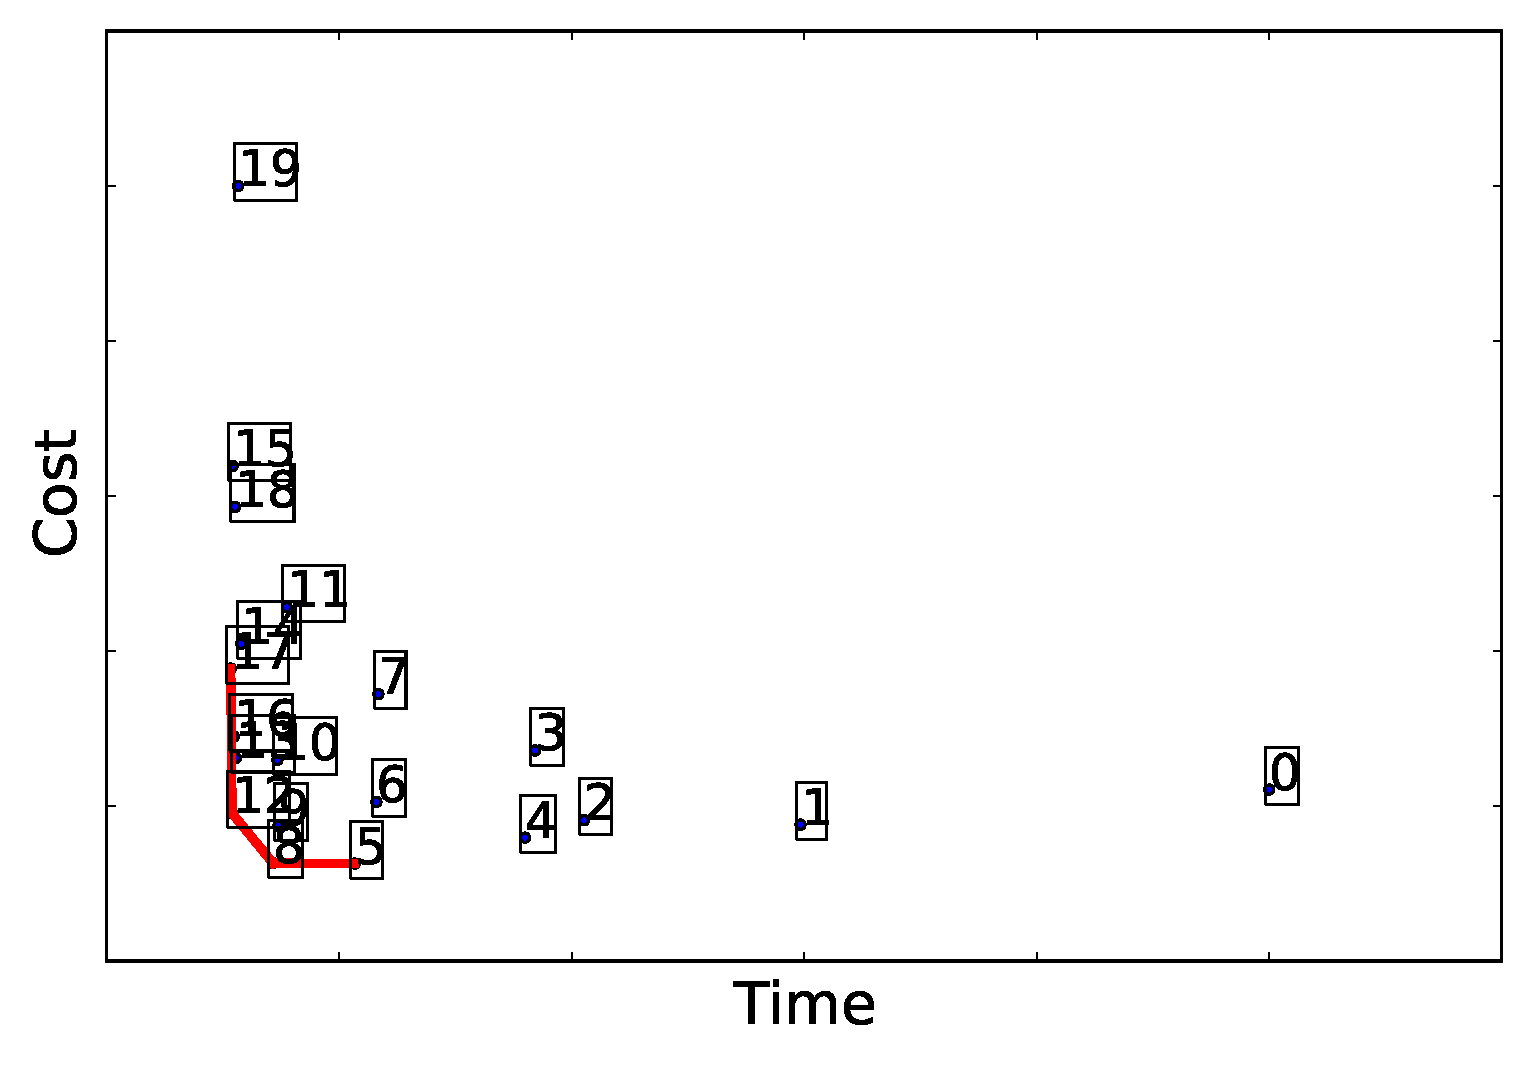
\includegraphics[width=\textwidth]{Chapter-CAT/figures/pagerank_elapsed_cost_all_frontier.eps}
        \caption{PageRank}
        \label{fig:pagerank_configurations}
    \end{subfigure}
    \begin{subfigure}[b]{0.3\textwidth}
        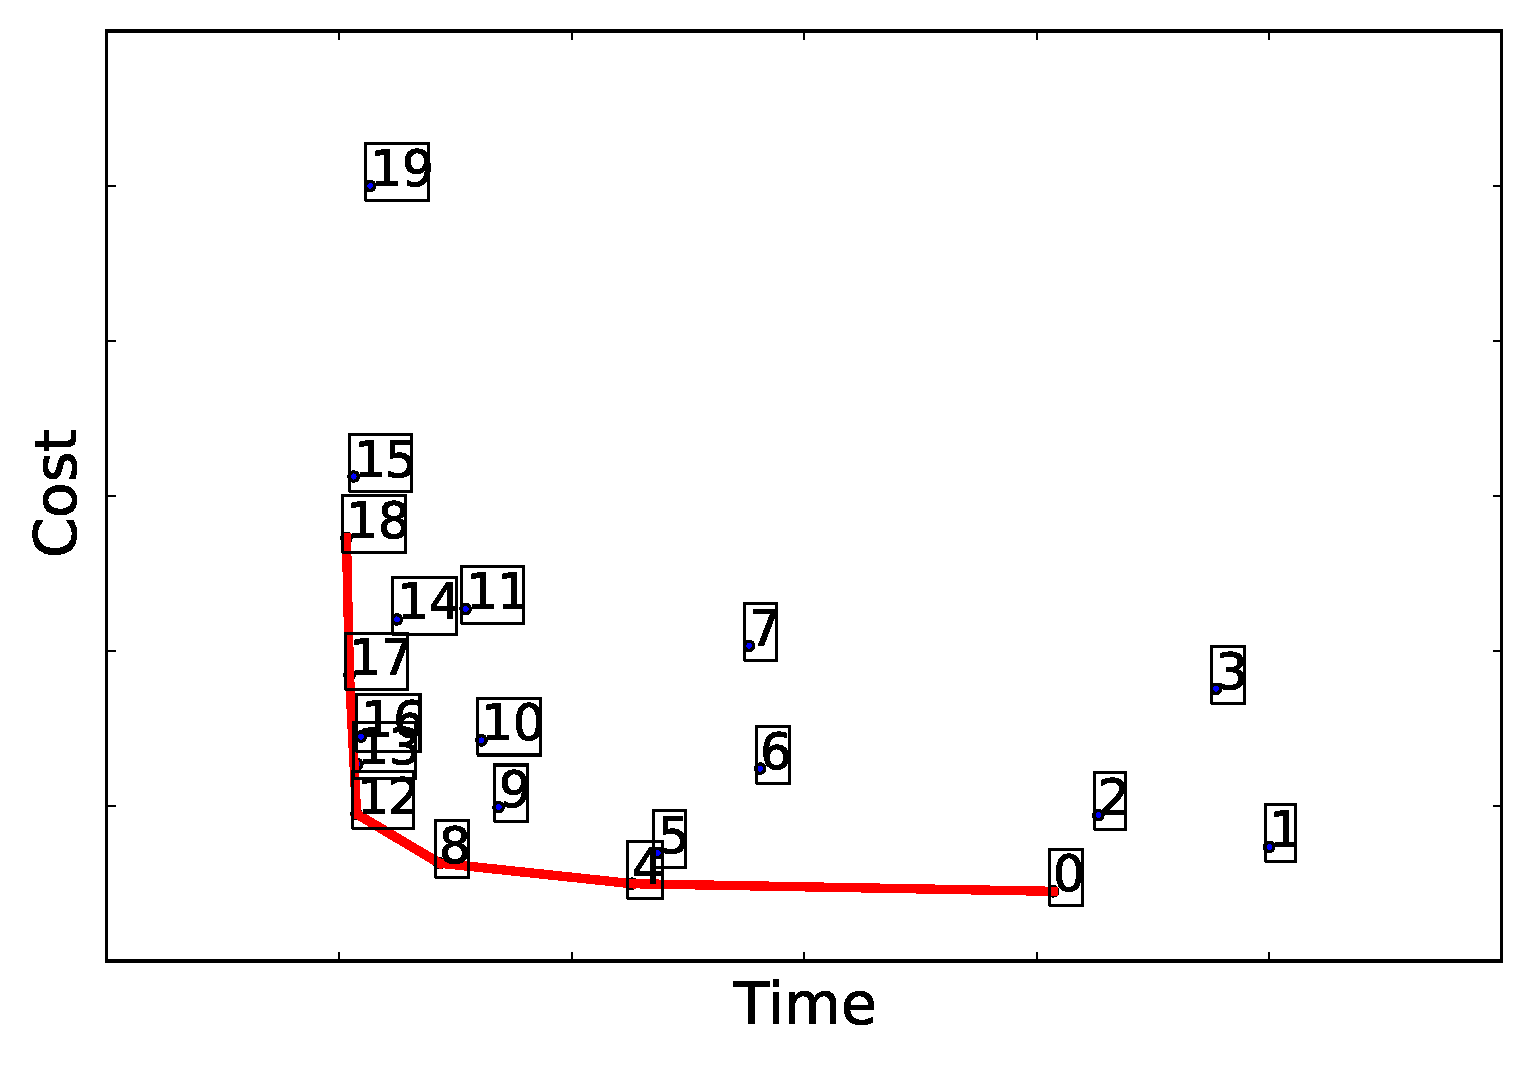
\includegraphics[width=\textwidth]{Chapter-CAT/figures/webloganalysis_elapsed_cost_all_frontier.eps}
        \caption{Web Log Analysis}
        \label{fig:webloganalysis_configurations}
    \end{subfigure}
    \begin{subfigure}[b]{0.3\textwidth}
        \includegraphics[width=\textwidth]{Chapter-CAT/figures/regression_elapsed_cost_all_frontier.eps}
        \caption{Regression}
        \label{fig:regression_configurations}
    \end{subfigure}
    \caption{Applications' execution time and resource costs with different configurations.}
    \label{fig:application_performance}
\end{figure}


\begin{figure}
    \captionsetup{justification=centering}
    \centering
    \begin{subfigure}[b]{0.3\textwidth}
        \includegraphics[width=\textwidth]{Chapter-CAT/figures/pagerank_cpu_elapsed_12_1.eps}
        \caption{PageRank}
        \label{fig:pagerank_time}
    \end{subfigure}
    \begin{subfigure}[b]{0.3\textwidth}
        \includegraphics[width=\textwidth]{Chapter-CAT/figures/webloganalysis_cpu_elapsed_12_1.eps}
        \caption{Web Log Analysis}
        \label{fig:webloganalysis_time}
    \end{subfigure}
    \begin{subfigure}[b]{0.3\textwidth}
        \includegraphics[width=\textwidth]{Chapter-CAT/figures/regression_cpu_elapsed_12_1.eps}
        \caption{Regression}
        \label{fig:regression_time}
    \end{subfigure}
    \bigskip
    \begin{subfigure}[b]{0.3\textwidth}
        \includegraphics[width=\textwidth]{Chapter-CAT/figures/pagerank_cpu_cost_12_1.eps}
        \caption{PageRank}
        \label{fig:pagerank_cost}
    \end{subfigure}
    \begin{subfigure}[b]{0.3\textwidth}
        \includegraphics[width=\textwidth]{Chapter-CAT/figures/webloganalysis_cpu_cost_12_1.eps}
        \caption{Web Log Analysis}
        \label{fig:webloganalysis_cost}
    \end{subfigure}
    \begin{subfigure}[b]{0.3\textwidth}
        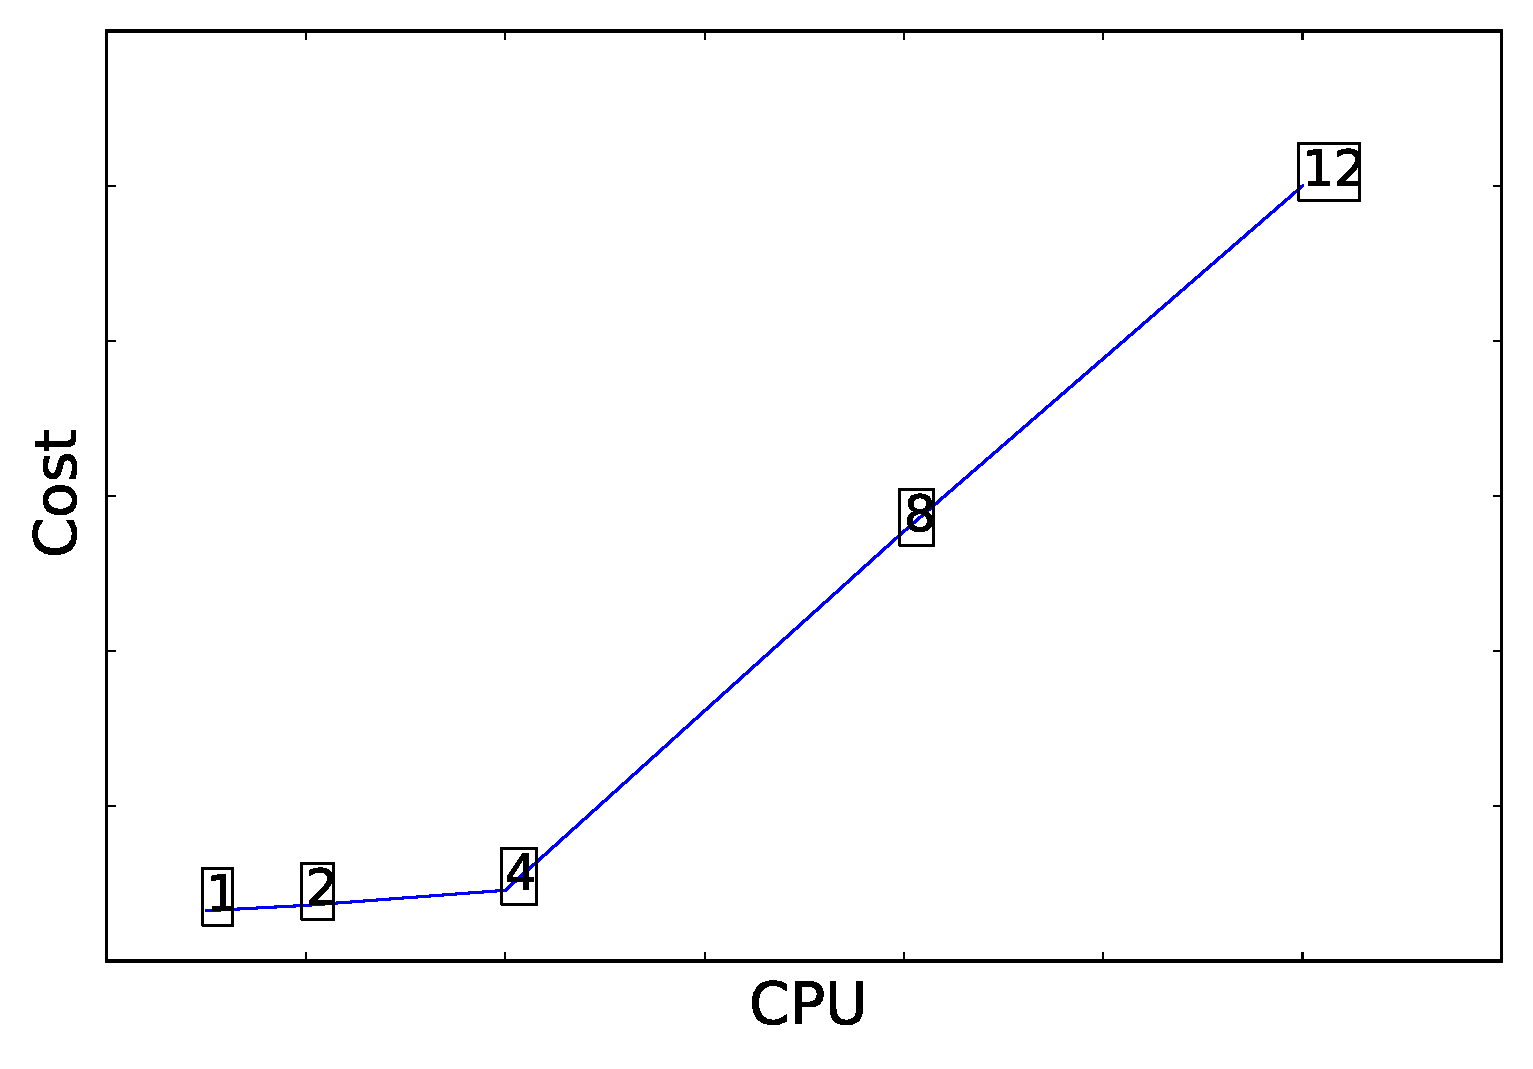
\includegraphics[width=\textwidth]{Chapter-CAT/figures/regression_cpu_cost_12_1.eps}
        \caption{Regression}
        \label{fig:regression_cost}
    \end{subfigure}
    \caption{The speedup and cost saving by CPU scaling (1GB memory per CPU).}
    \label{fig:speed_1gb}
\end{figure}





\iffalse
In this work, we focus on data processing jobs.
We are interested in two metrics:
1) how long to complete a job (execution \textbf{time})
\rone{at}
2) what \textbf{cost}.
Choosing the \emph{best} configuration is not always straightforward because
performance varies both between applications and across configurations within each application.
We run three real-world applications,
\emph{PageRank},
\emph{web log analysis}, and
\emph{regression},
on Apache Spark, a distributed, large-scale data processing system \cite{spark}.
We conduct a series of evaluations of the three applications against
different resource costs by varying
the number of CPUs (from 1 to 12)
and
the size of memory (from 1 to 4 GB per CPU).
We measure the execution time to complete the applications.
\mytable{\ref{table:raw_data}} lists their time and cost in detail.
\myfigure{\ref{fig:application_performance}} uses a scatter plot
to show 
the execution time of applications running against different resource \emph{costs}.
We find that their distribution patterns are not totally alike.
Therefore, there does not exist one best configuration for all applications.
Even within the same applications, execution time can change dramatically.
\myfigure{\ref{fig:application_performance}} also illustrates a convex hull
for outcomes bounded to a subset of the plane.
When choosing the \emph{best} configuration, the solution must be close to the
convex hull.

Finding out the most cost-effective configuration
is difficult for two reasons.
First, execution time is not linearly proportional to resource cost.
In \myfigure{\ref{fig:speed_1gb}}, we show that
the speedup is not linearly increasing with the number of CPUs.
Second, 
application performance is not monotonically increasing or decreasing
with respect to \emph{cost}.
\myfigure{\ref{fig:pagerank_cost}} demonstrates that
the \emph{PageRank} application is more cost-effective with four CPUs
even the cost per unit time is higher.
\emph{cost} is also a function of time.
When the time improvement is enough to compensate the cost increase,
cloud users are more willing to trade cost for time.

Our preliminary evaluation shows only two dimensions of configurations
, CPU and memory.
When it comes to real-world cloud deployment,
users need to figure out the \emph{best} configuration from
a larger dimension.
It is a time-consuming process and it is prone to mis-configuration,
which yields to deadline misses or higher charges.


\begin{table}[!htbp]
\centering
\caption{The execution time and resource cost of applications
running with different numbers of CPUs and memory per CPU.
The text in bold refer to the configurations on the convex hull
in \myfigure{\ref{fig:application_performance}}.}
\label{table:raw_data}
\begin{tabular}{rrrrrrrrr}
\multicolumn{3}{c}{\textbf{Configuration}}  & \multicolumn{2}{c}{\textbf{PageRank}} & \multicolumn{2}{c}{\textbf{Web Log Analysis}} & \multicolumn{2}{c}{\textbf{Regression}}\\
ID  & CPU & Memory/CPU & Time & Cost & Time & Cost & Time & Cost \\ \hline \hline
0   & 1          & 1       & 652.2 & 3261.1  & \textbf{179.3} & \textbf{896.3}  & \textbf{765.0}  & \textbf{3825.2} \\
1   & 1          & 2       & 389.2 & 2335.3  & 220.2 & 1321.1 & 706.7  & 4240.1 \\
2   & 1          & 4       & 267.7 & 2141.8  & 187.8 & 1502.4 & 723.7  & 5789.7 \\
3   & 1          & 8       & 240.3 & 2883.6  & 210.1 & 2521.1 & 701.0  & 8412.0 \\ \hline
4   & 2          & 1       & 234.6 & 2346.3  & \textbf{99.5}  & \textbf{994.6}  & \textbf{423.4}  & \textbf{4233.6} \\
5   & 2          & 2       & \textbf{139.1} & \textbf{1669.1}  & 104.3 & 1252.0 & 433.3  & 5200.1 \\
6   & 2          & 4       & 151.3 & 2420.0  & 123.8 & 1980.1 & 407.8  & 6524.6 \\
7   & 2          & 8       & 152.4 & 3657.0  & 121.6 & 2919.5 & 434.0  & 10414.2 \\ \hline
8   & 4          & 1       & \textbf{93.2}  & \textbf{1864.5}  & \textbf{63.0}  & \textbf{1259.5} & \textbf{269.1}  & \textbf{5382.2} \\
9   & 4          & 2       & 96.2  & 2310.0  & 74.2  & 1781.1 & \textbf{261.7}  & \textbf{6280.3} \\
10  & 4          & 4       & 95.7  & 3063.2  & 71.0  & 2270.8 & 268.7  & 8598.7 \\
11  & 4          & 8       & 101.0 & 4846.5  & 68.0  & 3262.1 & 275.9  & 13242.1 \\ \hline
12  & 8          & 1       & \textbf{70.3}  & \textbf{2811.5}  & \textbf{47.3}  & \textbf{1892.5} & 817.8  & 32711.8 \\
13  & 8          & 2       & 72.4  & 3475.4  & 47.5  & 2277.8 & 842.3  & 40431.1 \\
14  & 8          & 4       & 75.4  & 4828.5  & 55.0  & 3515.8 & 711.2  & 45518.7 \\
15  & 8          & 8       & 70.7  & 6783.4  & 46.8  & 4488.7 & 692.7  & 66502.3 \\ \hline
16  & 12         & 1       & 71.2  & 4272.9  & 48.1  & 2887.0 & 983.5  & 59007.1 \\
17  & 12         & 2       & \textbf{69.6}  & \textbf{5007.7}  & \textbf{46.0}  & \textbf{3309.2} & 1043.4 & 75122.3 \\
18  & 12         & 4       & 72.0  & 6912.8  & \textbf{45.4}  & \textbf{4357.1} & 1026.6 & 98549.5 \\
19  & 12         & 8       & 73.7  & 10617.9 & 49.9  & 7180.6 & 940.0  & 135362.0
\end{tabular}
\end{table}






\begin{figure}
	\captionsetup{justification=centering}
    \centering
	\begin{subfigure}[b]{0.3\textwidth}
        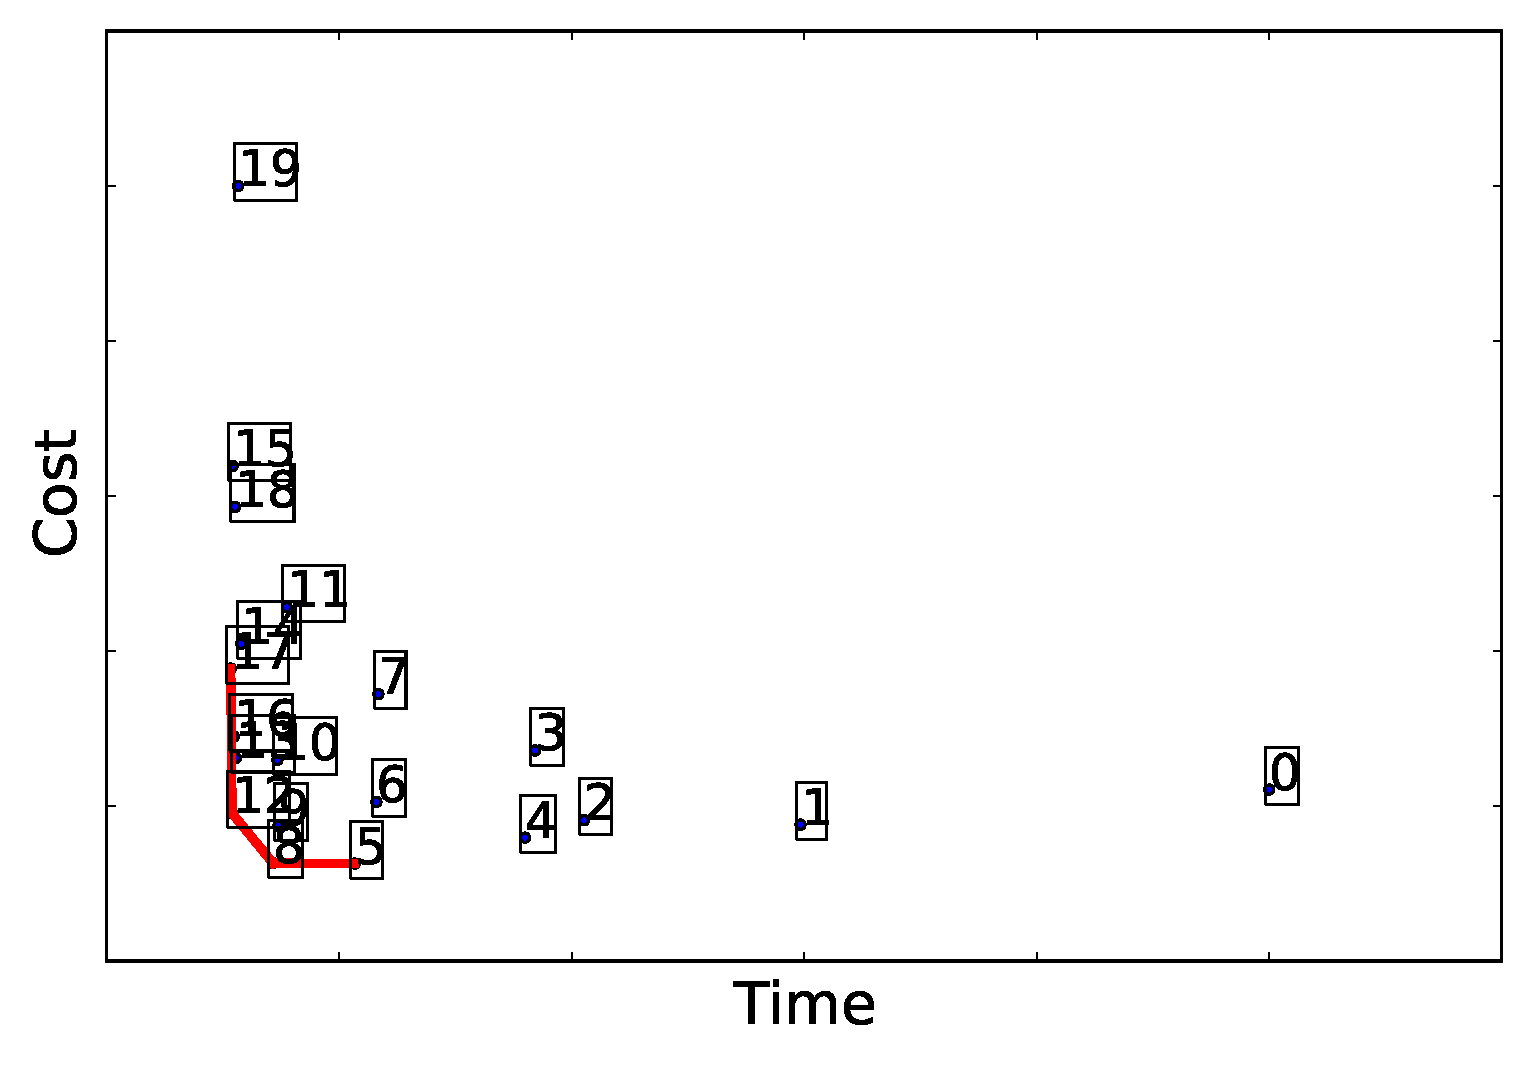
\includegraphics[width=\textwidth]{Chapter-CAT/figures/pagerank_elapsed_cost_all_frontier.eps}
        \caption{PageRank}
        \label{fig:pagerank_configurations}
    \end{subfigure}
    \begin{subfigure}[b]{0.3\textwidth}
        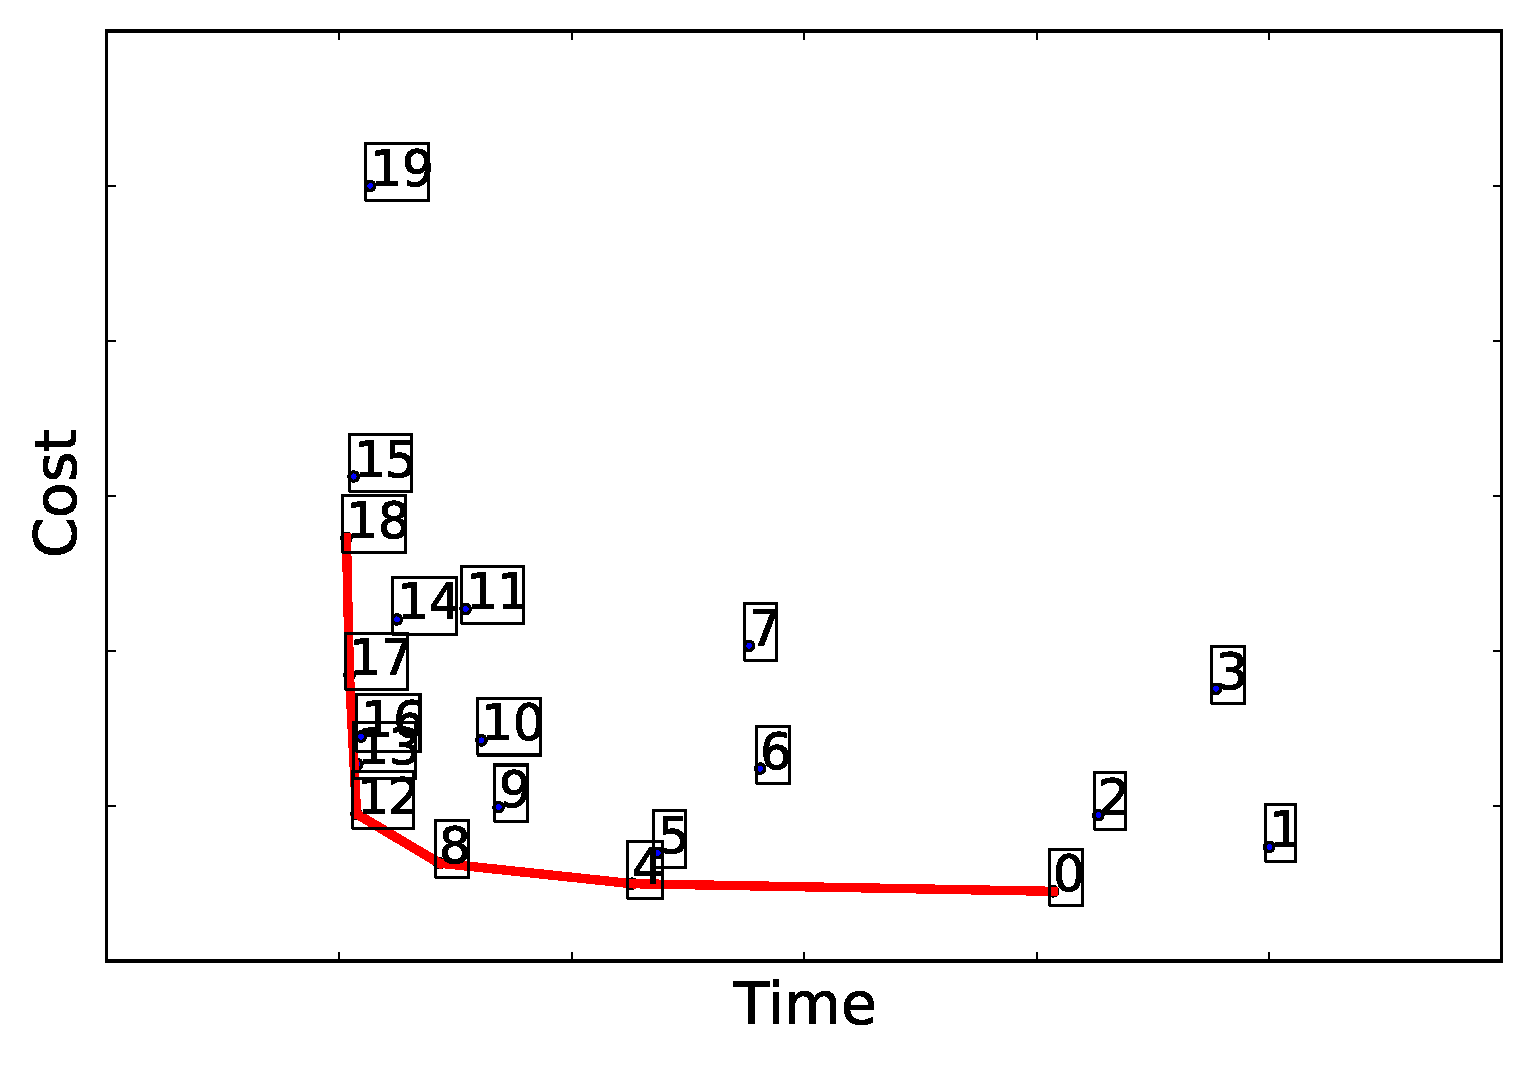
\includegraphics[width=\textwidth]{Chapter-CAT/figures/webloganalysis_elapsed_cost_all_frontier.eps}
        \caption{Web Log Analysis}
        \label{fig:webloganalysis_configurations}
    \end{subfigure}
    \begin{subfigure}[b]{0.3\textwidth}
        \includegraphics[width=\textwidth]{Chapter-CAT/figures/regression_elapsed_cost_all_frontier.eps}
        \caption{Regression}
        \label{fig:regression_configurations}
    \end{subfigure}
    \caption{Applications' execution time and resource costs with different configurations.}
    \label{fig:application_performance}
\end{figure}


\begin{figure}
	\captionsetup{justification=centering}
    \centering
	\begin{subfigure}[b]{0.3\textwidth}
        \includegraphics[width=\textwidth]{Chapter-CAT/figures/pagerank_cpu_elapsed_12_1.eps}
        \caption{PageRank}
        \label{fig:pagerank_time}
    \end{subfigure}
    \begin{subfigure}[b]{0.3\textwidth}
        \includegraphics[width=\textwidth]{Chapter-CAT/figures/webloganalysis_cpu_elapsed_12_1.eps}
        \caption{Web Log Analysis}
        \label{fig:webloganalysis_time}
    \end{subfigure}
    \begin{subfigure}[b]{0.3\textwidth}
        \includegraphics[width=\textwidth]{Chapter-CAT/figures/regression_cpu_elapsed_12_1.eps}
        \caption{Regression}
        \label{fig:regression_time}
    \end{subfigure}
    \bigskip
    \begin{subfigure}[b]{0.3\textwidth}
        \includegraphics[width=\textwidth]{Chapter-CAT/figures/pagerank_cpu_cost_12_1.eps}
        \caption{PageRank}
        \label{fig:pagerank_cost}
    \end{subfigure}
    \begin{subfigure}[b]{0.3\textwidth}
        \includegraphics[width=\textwidth]{Chapter-CAT/figures/webloganalysis_cpu_cost_12_1.eps}
        \caption{Web Log Analysis}
        \label{fig:webloganalysis_cost}
    \end{subfigure}
    \begin{subfigure}[b]{0.3\textwidth}
        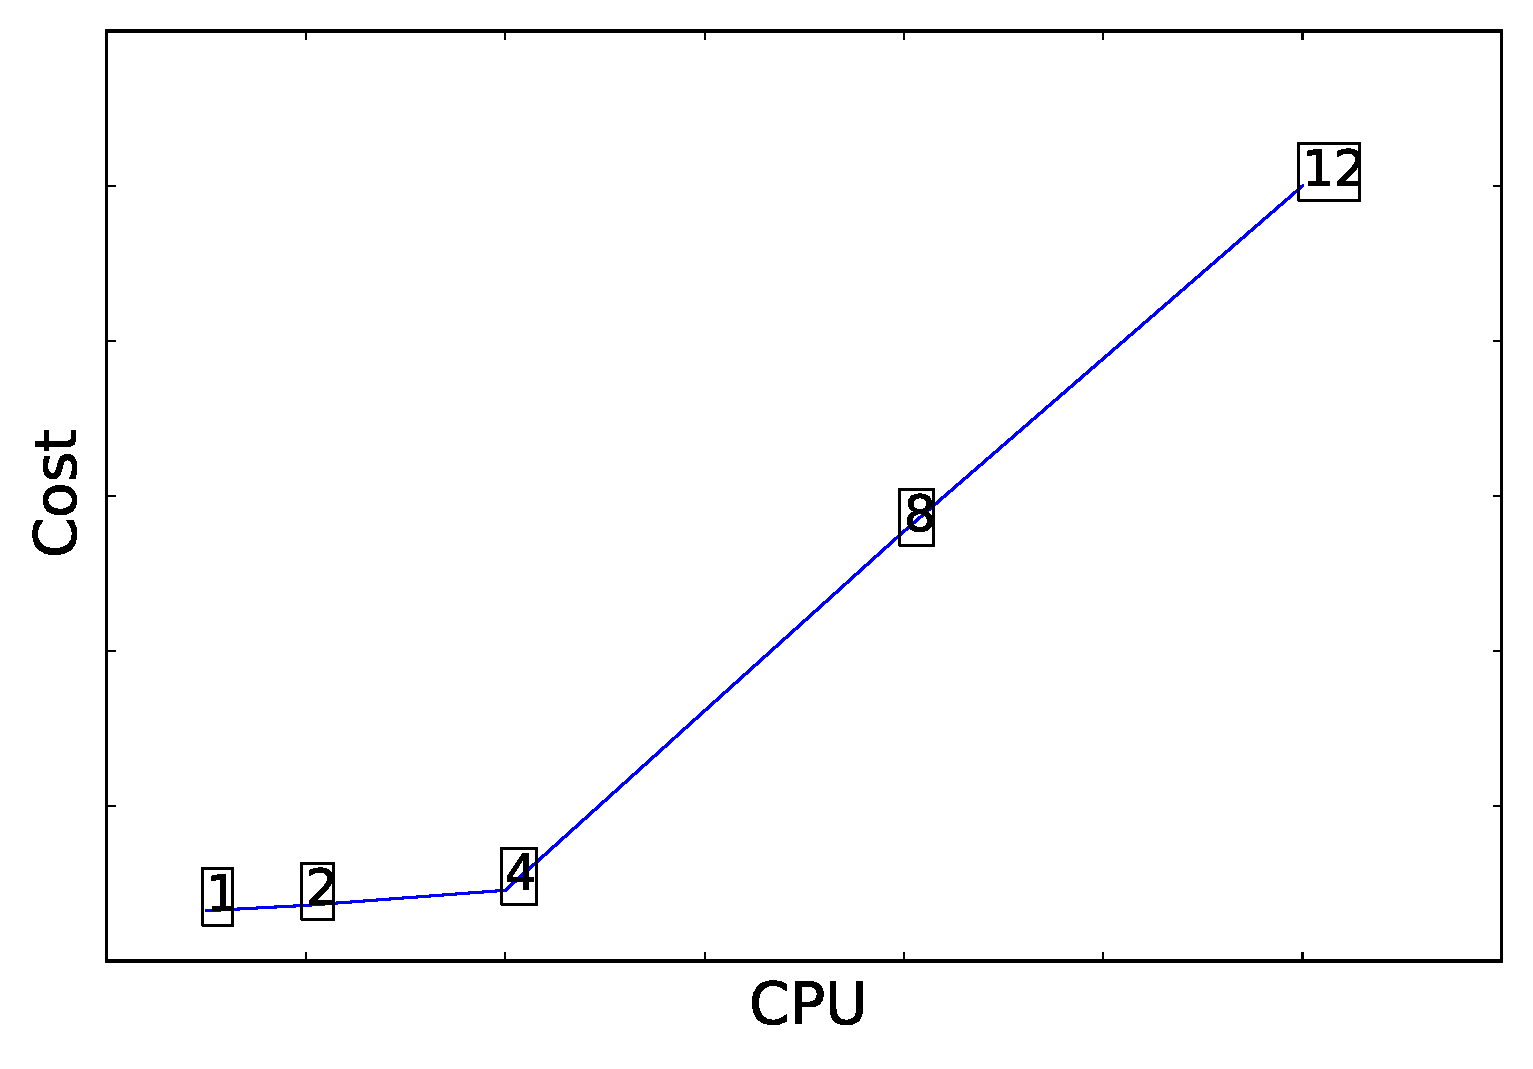
\includegraphics[width=\textwidth]{Chapter-CAT/figures/regression_cpu_cost_12_1.eps}
        \caption{Regression}
        \label{fig:regression_cost}
    \end{subfigure}
    \caption{The speedup and cost saving by CPU scaling (1GB memory per CPU).}
    \label{fig:speed_1gb}
\end{figure}


\paragraph*{Cost-Delay Product (CDP)}

When hosting data-intensive applications on the cloud,
users can choose the \emph{fastest} configuration regardless of cost
or the \emph{cheapest} configuration without the time constraint.
Neither choice is truly piratical.
There is always a trade-off between \emph{time} and \emph{cost}.
Users are willing to spend more on resources when
time is more critical (hard deadline) or
the increase in cost expects reasonable decrease in execution time (soft deadline).
Similarly, when the time constraint is relaxed, users accept
slower configuration but with higher cost saving.

We propose using cost-delay product (CDP),
similar to energy-delay product (EDP)~\cite{Freeh2007},
to analyze the trade-offs
for choosing the cloud configurations of data-intensive applications.
CDP puts the same importance on time and cost.
For example,
a $5\%$ slow down in execution time
is enough to justify
a $5\%$ cost saving.
$CD^2P$ and $C^2DP$, on the other hand, shift the importance to
time and cost respectively.
When the time improvement is $1\%$ but it incurs $50\%$ increase in cost,
users will probably choose the slower configuration.
In the PageRank case, for example,
users are more likely to choose four CPUs instead of eight CPUs because
25\% reduction in execution time requires
more than 50\% extra cost.
We explain the three applications' trade-off as follows.

\subparagraph*{PageRank}

PageRank is an ranking algorithm to calculate the importance of website pages
by counting the number of links to them.
Our evaluation has shown that execution time decreases as
we increase the number of CPUs.
Although \emph{PageRank} exhibits shorter execution time
when the CPU count is greater than eight,
it more makes sense to choose four CPUs as it is more cost effective,
as depicted in~\myfigure{\ref{fig:pagerank_cost}}.
However, when time is more critical ($CD^2P$),
~\myfigure{\ref{fig:pagerank_time}} shows that
eight CPUs is a better choice.

\subparagraph*{Web Log Analysis}
This application tracks the query counts and aggregate bytes in a particular group.
The CPU count greatly affects the execution time but memory size does not
show significant impact.
As shown in~\myfigure{\ref{fig:webloganalysis_time}}, a larger number of CPUs (increasing from 1 to 4)
increase resource costs but time reduction is large enough
to compensate the increase in cost.
This is not the case when the CPU count is more than four.
When time is more critical, $CD^2P$ suggests eight CPUs is a viable configuration.

\subparagraph*{Regression}
The regression application generates a function that estimates 
the relationships among variables.
Different from the above two applications, \emph{regression} shows
more CPU counts do no necessarily help reduce execution time.
It is even worse.
One possible explanation is the overhead by increasing parallelism overcomes
the benefits by higher parallelism.


\iffalse
\begin{figure}
	\captionsetup{justification=centering}
    \centering
	\begin{subfigure}[b]{0.3\textwidth}
        \includegraphics[width=\textwidth]{Chapter-8/figures/pagerank_cpu_CDP_12_1.eps}
        \caption{PageRank}
        \label{fig:pagerank_cdp}
    \end{subfigure}
    \begin{subfigure}[b]{0.3\textwidth}
        \includegraphics[width=\textwidth]{Chapter-8/figures/webloganalysis_cpu_CDP_12_1.eps}
        \caption{Web Log Analysis}
        \label{fig:webloganalysis_cdp}
    \end{subfigure}
    \begin{subfigure}[b]{0.3\textwidth}
        \includegraphics[width=\textwidth]{Chapter-8/figures/regression_cpu_CDP_12_1.eps}
        \caption{Regression}
        \label{fig:regression_cdp}
    \end{subfigure}
    \bigskip
    \begin{subfigure}[b]{0.3\textwidth}
        \includegraphics[width=\textwidth]{Chapter-8/figures/pagerank_cpu_CD2P_12_1.eps}
        \caption{PageRank}
        \label{fig:pagerank_cd2p}
    \end{subfigure}
    \begin{subfigure}[b]{0.3\textwidth}
        \includegraphics[width=\textwidth]{Chapter-8/figures/webloganalysis_cpu_CD2P_12_1.eps}
        \caption{Web Log Analysis}
        \label{fig:webloganalysis_cd2p}
    \end{subfigure}
    \begin{subfigure}[b]{0.3\textwidth}
        \includegraphics[width=\textwidth]{Chapter-8/figures/regression_cpu_CD2P_12_1.eps}
        \caption{Regression}
        \label{fig:regression_cd2p}
    \end{subfigure}
    \bigskip
    \begin{subfigure}[b]{0.3\textwidth}
        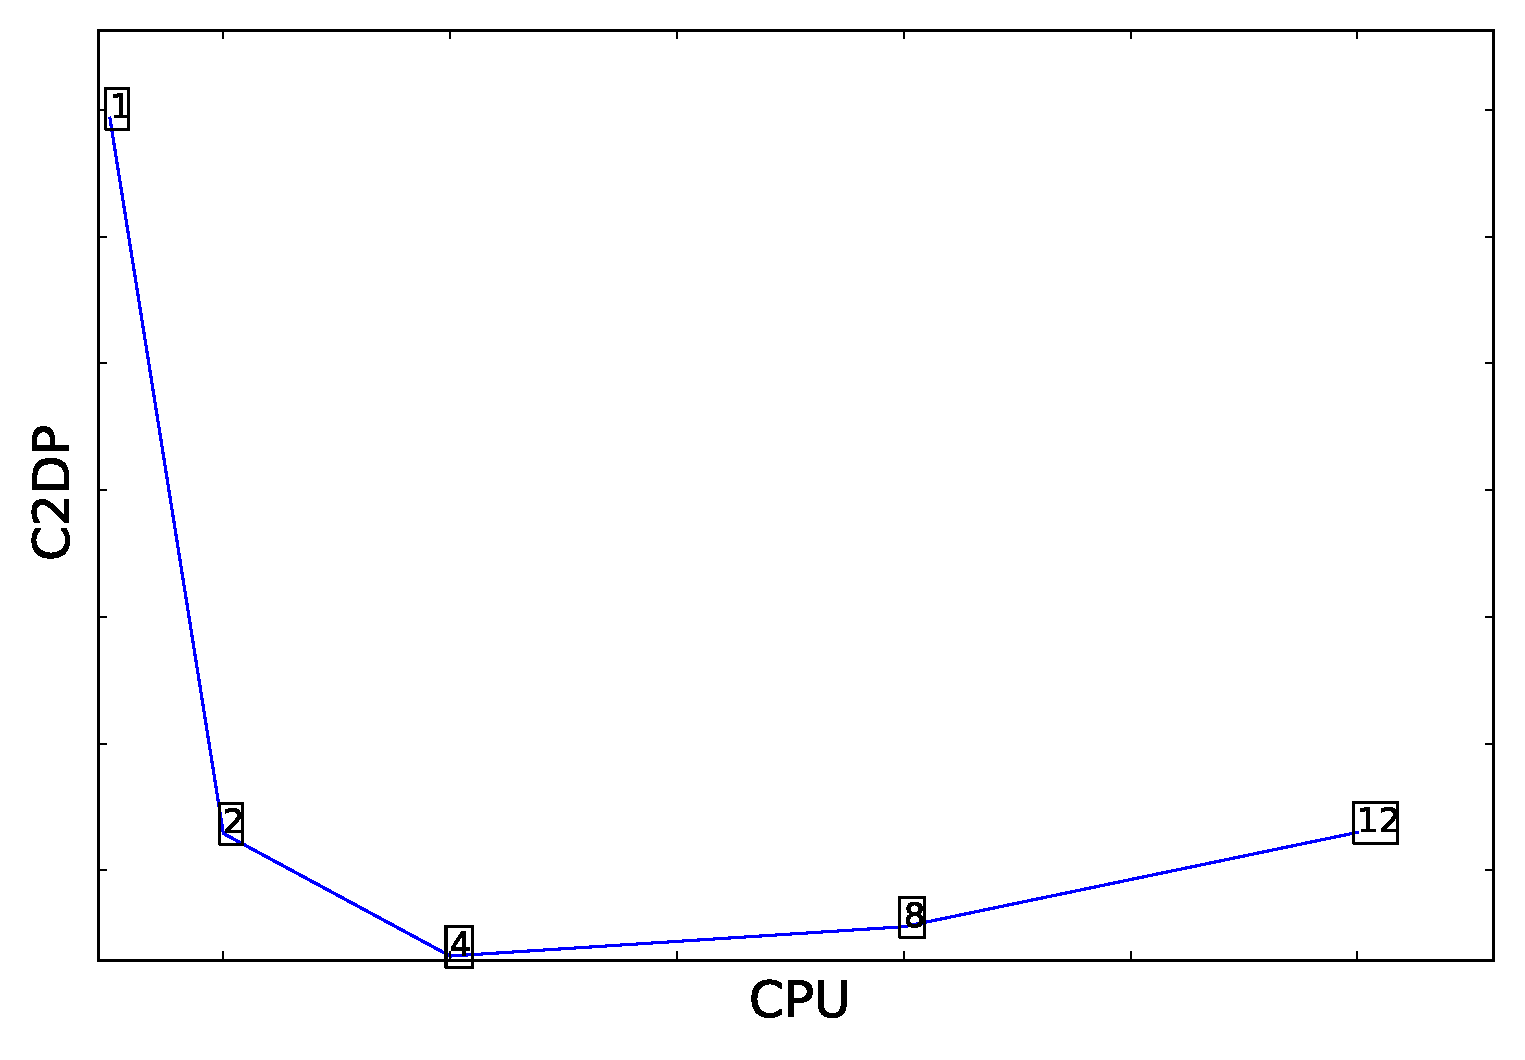
\includegraphics[width=\textwidth]{Chapter-8/figures/pagerank_cpu_C2DP_12_1.eps}
        \caption{PageRank}
        \label{fig:pagerank_c2dp}
    \end{subfigure}
    \begin{subfigure}[b]{0.3\textwidth}
        \includegraphics[width=\textwidth]{Chapter-8/figures/webloganalysis_cpu_C2DP_12_1.eps}
        \caption{Web Log Analysis}
        \label{fig:webloganalysis_c2dp}
    \end{subfigure}
    \begin{subfigure}[b]{0.3\textwidth}
        \includegraphics[width=\textwidth]{Chapter-8/figures/regression_cpu_C2DP_12_1.eps}
        \caption{Regression}
        \label{fig:regression_c2dp}
    \end{subfigure}
    \caption{CDP analysis for the cost and time trade-off}
    \label{fig:cdp_analysis}
\end{figure}
\fi



Our preliminary evaluations have shown that
it is not obvious to choose the \emph{best} configuration
because there is no clear relationship between \emph{time} and \emph{cost}.
Besides, applications have very different trade-off curves.
It requires a thorough understanding of application performance and resource capability
for finding out the most cost-effective configurations,
given a time and cost objectives.

\fi

